\documentclass[10pt,landscape]{article}
\usepackage{amssymb,amsmath,amsthm,amsfonts}
\usepackage{multicol,multirow}
\usepackage{calc}
\usepackage{graphicx}
\usepackage{ifthen}
\usepackage[landscape]{geometry}
\usepackage[colorlinks=true,citecolor=blue,linkcolor=blue]{hyperref}


\ifthenelse{\lengthtest { \paperwidth = 11in}}
    { \geometry{top=.33in,left=.33in,right=.33in,bottom=.33in} }
	{\ifthenelse{ \lengthtest{ \paperwidth = 297mm}}
		{\geometry{top=1cm,left=1cm,right=1cm,bottom=1cm} }
		{\geometry{top=1cm,left=1cm,right=1cm,bottom=1cm} }
	}
\pagestyle{empty}
\makeatletter
\renewcommand{\section}{\@startsection{section}{1}{0mm}%
                                {-1ex plus -.5ex minus -.2ex}%
                                {0.5ex plus .2ex}%x
                                {\normalfont\scriptsize\bfseries}}
\renewcommand{\subsection}{\@startsection{subsection}{2}{0mm}%
                                {-1explus -.5ex minus -.2ex}%
                                {0.5ex plus .2ex}%
                                {\normalfont\scriptsize\bfseries}}
\renewcommand{\subsubsection}{\@startsection{subsubsection}{3}{0mm}%
                                {-1ex plus -.5ex minus -.2ex}%
                                {1ex plus .2ex}%
                                {\normalfont\scriptsize\bfseries}}
\makeatother
\setcounter{secnumdepth}{0}
\setlength{\parindent}{0pt}
\setlength{\parskip}{0pt plus 0.5ex}
% -----------------------------------------------------------------------

\title{COMPSCI 2GA3 - Geon}

\begin{document}

\raggedright
\footnotesize

%\begin{center}
%     \Large{\textbf{COMPSCI 2GA3 - Geon}} \\
%\end{center}
\tiny\begin{multicols}{3}
\setlength{\premulticols}{1pt}
\setlength{\postmulticols}{1pt}
\setlength{\multicolsep}{3pt}
\setlength{\columnsep}{2pt}

\section{Digital logic}
%{\centering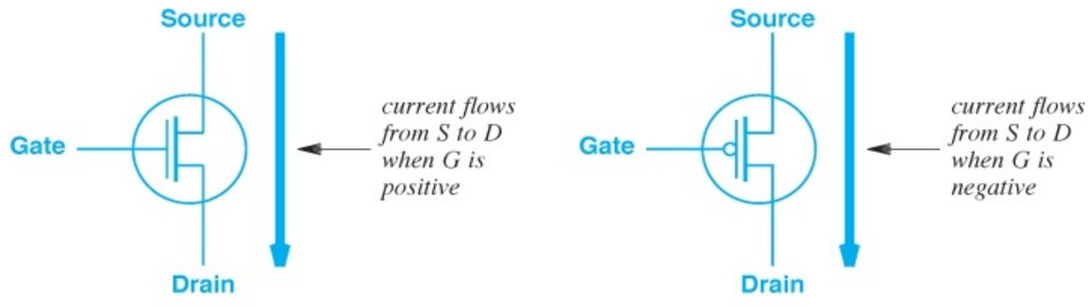
\includegraphics[scale=0.23]{img/trans.png}\par}
{\centering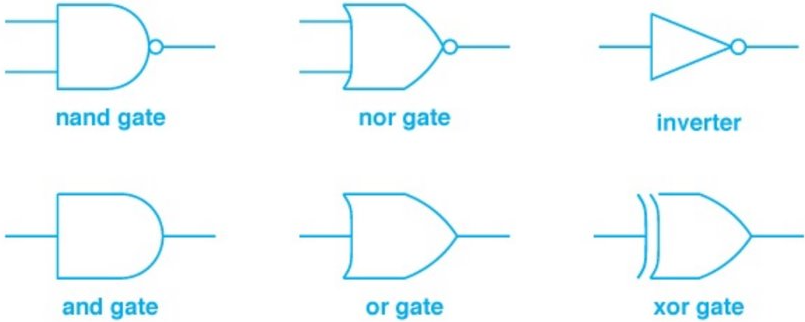
\includegraphics[scale=0.23]{img/lg.png}\par} 
\textbf{Half adder}: takes two input bits, outputs sum (xor) and carry (and).\\
%{\centering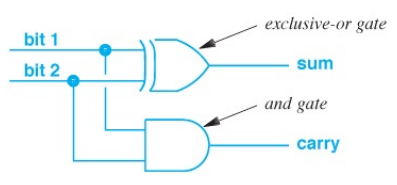
\includegraphics[scale=0.29]{img/had.png}\par} 
\textbf{Full adder}: takes two input bits and a carry, outputs sum and carry. Built from two half adders and an or gate.\\
%{\centering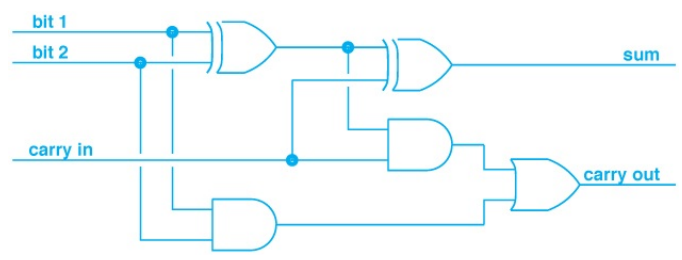
\includegraphics[scale=0.28]{img/fad.png}\par} 
\textbf{Latch}: uses previous output until the enable line is enabled. The output remains the same (even when the enable line is on) until propagation delay is over.\\
%{\centering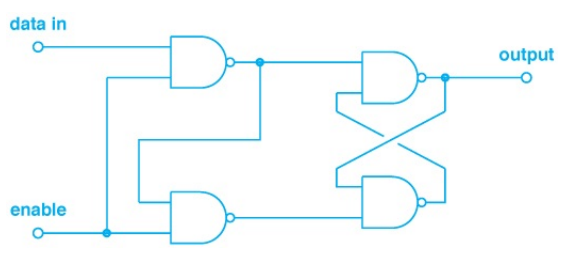
\includegraphics[scale=0.3]{img/l.png}\par}
\textbf{Propagation delay}: the delay between an input change an an output change.\\
%\textbf{Register}: stores bits through a series of latches. Different types: general-purpose, floating point, instruction pointer, comparison operation. Use to load data from memory to register, perform ALU operation, and store result from register to memory. \\
%{\centering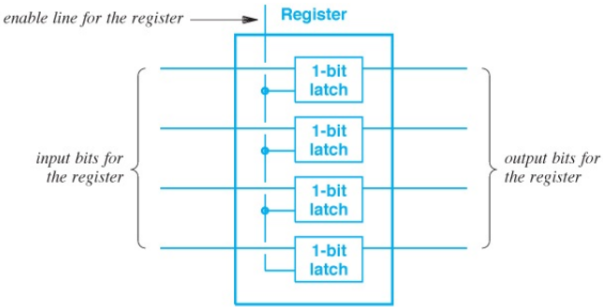
\includegraphics[scale=0.4]{img/register.png}\par}
%\textbf{Binary counter}: counts in binary. Takes in 1 input, and with $n$ outputs, it can count from $0$ to $2^n-1$. When the input \textit{goes from 0 to 1}, the counter increments by 1. It can have more inputs for \textit{reset} and \textit{pause}. It can have more outputs for \textit{overflow}.\\
%\textbf{Clock}: controls a logic circuit, allowing components to operate without requiring input to change. Oscillates at a regular rate between 1 and 0. \textit{Clocked} components can be synchronized and work as a function of its inputs \textit{and time}.\\
%\textbf{Decoder}: takes in a $n$-bit binary value and enables one of $2^n$ outputs.\\
%{\centering{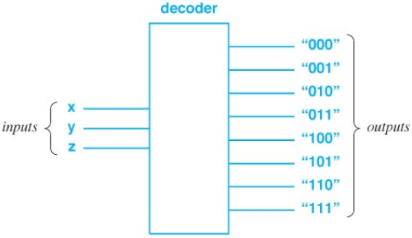
\includegraphics[scale=0.5]{img/decoder.png}}\par}
%\textbf{Demultiplexor}: a decoder that takes an extra input which gets passed to the selected output. 
\section{Representations}
%\textbf{Bit}: 0 or 1.\\
%\textbf{Byte}: group of bits (usually 4).\\
%\textbf{Word}: group of bytes (usually 2).\\
%\textbf{Big endian}: MSB to LSB (i.e. how we usually read numbers).\\
%\textbf{Little endian}: LSB to MSB.\\
\textbf{Unsigned integers}: only positive integers from $0$ to $2^k-1$.\\
\textbf{Sign-magnitude}: MSB is sign, rest is magnitude. From $0$ to $2^{k-1}-1$ and from $-0$ to $-2^{k-1}-1$.\\
\textbf{One's complement}: MSB is sign, rest is magnitude. Flipped for negative. From $0$ to $2^{k-1}-1$ and from $-0$ to $-2^{k-1}-1$.\\
\textbf{Two's complement}: MSB is sign, rest is magnitude. Flipped - 1 for negative. From $0$ to $2^{k-1}-1$ and from $-1$ to $-2^{k-1}$.\\
\textbf{Floating-point (IEEE)}: stored as \texttt{sign-exponent-mantissa}: $(-1)^s\cdot(1+m)\cdot 2^{e-b}$ where $s$ is the sign, $m$ is the mantissa, $e$ is the biased exponent and $b$ is the bias. The exponent is biased so it can have negative numbers while being unsigned: $b=2^{k-1}-1$ where $k$ is the number of bits the exponent has. So, $e'=e+b$ where $e$ is the unbiased exponent. The mantissa is \textit{normalized} and is assumed to start with 1.
%\textbf{Binary coded decimal}: encode every decimal digit in a byte (4 bits). For fractions, either include an explicit decimal point in the string or specify its location. For signs, a \texttt{0xD} is put at the end to indicate it's negative. 
\section{Processors}
\textbf{Von Neumann architecture}: single memory to hold both instructions and data. More flexible, but bottleneck between memory to processor. More popular than Harvard.\\
%{\centering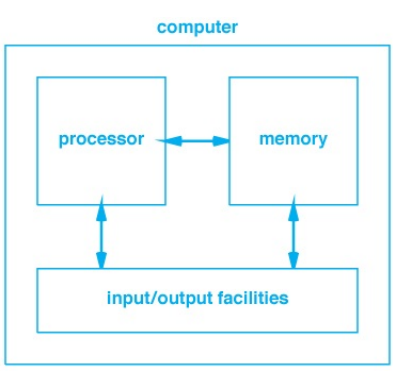
\includegraphics[scale=0.35]{img/vna.png}\par}
\textbf{Harvard architecture}: separate memory for instructions and data. Less susceptible to bottlenecks and more secure, but the split between instructions and data memory is rigid.\\
%{\centering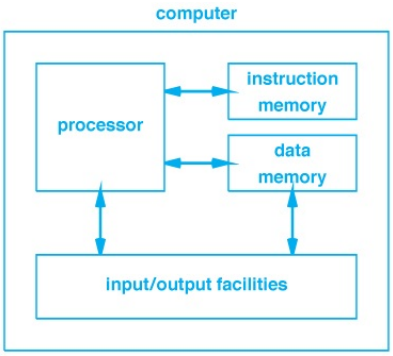
\includegraphics[scale=0.35]{img/ha.png}\par}
\textbf{Processor}: a digital device that can perform multi-step computation.\\
\textbf{Types}:
\begin{itemize}
\item \textbf{Fixed logic}: function is fixed in hardware.
\item \textbf{Selectable logic}: can choose one of several fixed functions.
\item \textbf{Parameterizable logic}: parameters control computation of fixed functions.
\item \textbf{Programmable logic}: list of instructions provided at runtime.
\end{itemize}
\textbf{Categories}:
\begin{itemize}
\item\textbf{Co-processors}: dedicated function; fixed/selectable logic.
\item\textbf{Microcontrollers}: programmable logic, direct hardware control.
\item\textbf{Embedded systems}: real-time OS, dedicated hardware.
\item\textbf{General purpose}: more functionality than embedded systems.
\end{itemize}
\textbf{Units}:
\begin{itemize}
\item\textbf{Controller}: controls the flow of program execution.
\item\textbf{Arithmetic logic unit}: performs all computational tasks sequentially according to controller.
\item\textbf{Local storage (registers)}: holds data values.
\item\textbf{Internal connections}: Transfers data values between hardware units (between local storage and ALU).
\item\textbf{External interface}: handles communication between processors and the rest of the computer system.
\end{itemize}
\subsection{Fetch-execute cycle}
The \textit{instruction pointer} \texttt{ip} automatically moves through the program in memory. The cycle \textit{doesn't proceed at a fixed rate} since execution speed depends on the instruction. The cycle \textit{never ends} (unless the system powers down) so there always needs to be a program executing (either the same program or OS).
%\begin{verbatim}
%ip = start of program
%repeat forever
%    instruction = fetch(memory[ip++])
%    execute instruction
%\end{verbatim}
\section{Instructions}
%Usually encoded as \texttt{opcode-operands-offset}.\\
\textbf{Instruction sets}: the \textit{design} of all available instructions for a processor (available instructions, what each instruction does, number of operands, operand encoding, instruction encoding, result storing, etc).\\
\textbf{Branching}: moving the \textit{instruction pointer} to a different location in the program (e.g. for conditionals, loops, etc.).
%\begin{verbatim}
%ip = start of program
%repeat forever
%    instruction = fetch(memory[ip])
%    tmp = ip + 1
%    execute instruction
%    ip = tmp
%\end{verbatim}
%\textbf{Absolute branching}: \texttt{tmp = absolute address}\\
%\textbf{Relative branching}: \texttt{tmp = ip + offset}\\
\textbf{Register bank}: each \textit{bank} stores a set of registers. Allows parallel access to different registers within the same clock cycle. Can lead to register bank conflicts if an operation requires multiple registers from the same bank. \\
%\textbf{Subroutine}: another word for branching. \\
\textbf{Passing arguments to subroutine calls}: either stored in \textit{memory} or \textit{registers} through \textit{register windows}.\\
\textbf{Register window}: exposing only a set of registers at a time (i.e. a window), which moves each time a subroutine is called and moves back when it returns. The window overlaps with what the program sees and what the subroutine sees so \textit{arguments are passed into the overlapping registers}.\\
%{\centering 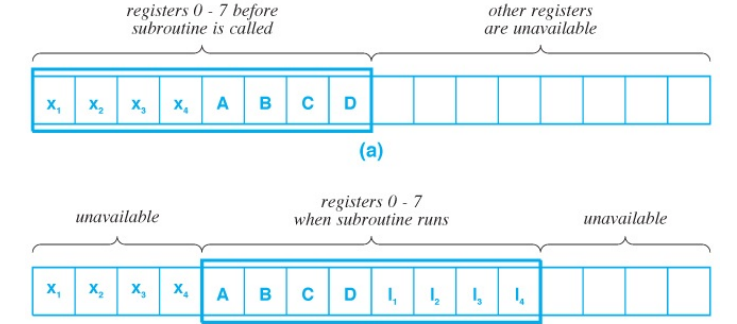
\includegraphics[scale=0.4]{img/rw.png}\par}
\textbf{Complex instruction set computer (CISC)}: a kind of ISA where each instruction performs a \textit{complex operation}, instructions take \textit{variable number} of clock cycles, and requires \textit{fewer instruction calls} than a RISC.\\
\textbf{Reduced instruction set computer (RISC)}:  a kind of ISA where each instruction performs a \textit{simple operation}, instructions take the \textit{same number} of clock cycles (achieved through the RISC pipeline), and requires \textit{many instruction calls}.\\	
%\textbf{Throughput}: the amount of work done per unit time.\\
\textbf{Pipeline}: a computational architecture that improves throughput if computation can be divided into \textit{distinct stages}, each stage takes \textit{similar time} to complete, and it's \textit{efficient} to move data between stages.\\
\textbf{RISC pipeline}: a 5 stage pipeline for RISC that allows one instruction to execute per clock cycle \textbf{once the pipeline is filled}.\\
{\centering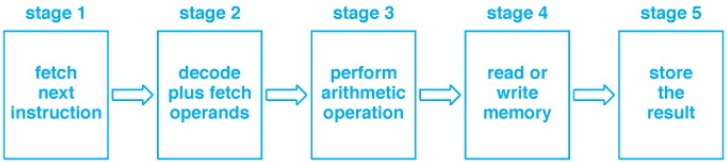
\includegraphics[scale=0.39]{img/rp.png}\par}
\textbf{Stall}: disrupts the flow of a pipeline. Creates a \textit{bubble} that floats until the pipeline restarts. Also called a \textit{hazard}.\\
\textbf{Bubble}: a delay in the pipeline of one or more clock cycles due to a stall.\\
\textbf{Data hazard}: a stall from an instruction \textit{waiting for data} from an earlier instruction. Solved by \textit{forwarding} between stages or \textit{rearranging instructions} so instructions requiring data from earlier instructions occur later. \\
\textbf{Forwarding}: pass results from earlier instructions into later instructions that require it \textit{right after it's calculated} rather than once it's done being stored.\\
\textbf{Control hazard}: a stall from an \textit{incorrect instruction} in the pipeline, causing \textit{branching}. Solved by predicting conditional branching and flushing the pipeline if the prediction is wrong.\\
\textbf{Structural hazard}: a stall from \textit{resource conflicts} where a required resource is needed simultaneously by more than one instruction. Solved by loading data in parallel like in \textit{register banks}.\\
\subsection{Operands}
The arguments of instructions. Can either be \texttt{src} (value, register, address) or \texttt{dst} (register, address).\\
There can be \textit{fixed} (bit fields have same semantics) and \textit{variable} (more memory efficient) number of operands. \\
\begin{enumerate}
\item \textbf{0 operands}: stack architecture.
\item \textbf{1 operands}: implicit destination.
\item \textbf{2 operands}: specified destination, given operand is destination.
\item \textbf{3 operands}: specified destination, can have separate destination from inputs.
\end{enumerate}
\textbf{Implicit encoding}: opcodes define what type of operands we need.\\
\textbf{Explicit encoding}: operand fields define what type of operands.\\
\textbf{Different ways operands can be accessed}:
\begin{enumerate}
\item \textit{Immediate value} in instruction.
\item Value in register, \textit{register id} in instruction.
\item Value in memory, \textit{memory address} in instruction.
\item Value in memory, \textit{memory address in register}, register id in instruction. I.e. pointer.
\item Value in memory, memory address in \textit{different memory location} encoded in instruction. I.e. double pointer.
\end{enumerate}
\section{Microcode}
CPU and programmer views the macro instruction set, which is implemented with microcode that is hidden to the programmer. Micro instruction set is implemented with digital logic and is processed by the microcontroller.\\
\textbf{Pros}: less prone to errors compared to hardware design; easier to implement; ease of extension and modification; offers another level of abstraction.\\
\textbf{Cons}: more overhead than dedicated hardware design; variable cost for macro instructions (depends on number of micro instructions); microcontroller needs to run very fast.\\
\textbf{Vertical microcode}: sequential coding where you control one functional unit at a time. Microcontroller runs the instructions in sequence. More intuitive.\\
\textbf{Horizontal microcode}: each instruction is a bit string that controls multiple functional units simultaneously. Some operations can take multiple cycles and you have to tell the ALU to \texttt{continue}. As long as resources aren't blocked, parallel execution is possible.\\
\textbf{Lookahead execution}: microcontroller can look ahead to next instruction and perform optimization at the micro instruction level, but need to preserve computation semantics (result of computation stays the same). Lookahead for conditional branching does branch prediction or execution depending on hardware.
\subsection{Compilation}
High-level languages are \textit{compiled} into binary \textit{object code} for the processor to compute through the fetch-execute cycle. 
\begin{enumerate}
\item \textbf{Preprocessor}: expands macros.
\item \textbf{Compiler}: translates to assembly language.
\item\textbf{Assembler}: translates to relocatable object code (contains references to external library functions).
\item \textbf{Linker}: replaces external function references with its code.
\end{enumerate}
{\centering 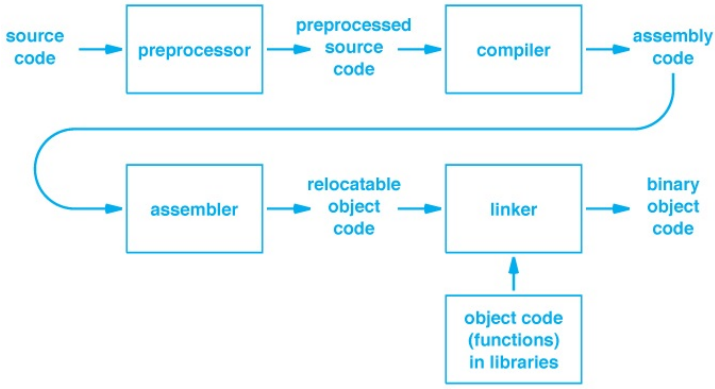
\includegraphics[scale=0.35]{img/c.png}\par}
\textbf{High-level language}: one line to many instruction translation; hardware independent (can be  compiled in either x86-64 or ARM); usability: application oriented, general purpose, and powerful abstractions.\\
\textbf{Low-level language}: one line to one instruction translation; hardware specific (code is specific to x86-64 or ARM); usability: systems programming oriented, special purpose, and few abstractions.\\
\textbf{Two-stage assembler}: a kind of assembler for assembly where step 0 is running the preprocessor; step 1 is mapping each instruction to a memory address and building a label symbol table; and step 2 is translating instructions into binary and substituting labels with their location in the symbol table.
\section{Physical memory}
\textbf{Memory}: any physical storage device that can \textit{store and retrieve} information. CPU doesn't get memory directly, it asks the memory controller (a microcontroller).\\
\textbf{Volatile}: when power is off, values are gone (e.g. RAM).\\
\textbf{Persistent}: maintain values when power is off (e.g. SSD, HDD).\\
\textbf{Random access}: cost of memory access is the same regardless of the location in memory (e.g. RAM).\\
\textbf{Sequential}: order matters in cost of memory access (e.g. CD). Includes a location pointer, which requires time to go from A to B.\\
\textbf{Access rights}: read-write vs. read-only.\\ 
\textbf{Primary}: computer's main memory and stores data temporarily (e.g. RAM and registers).\\
\textbf{Secondary}: external memory and saves data permanently (e.g. SSD, HDD).\\
\textbf{Density}: how much data can we store per unit chip area?\\
\textbf{Latency}: time to complete a single operation.\\
\textbf{Cycle time}: average time per operation.\\
\textbf{Clock frequency}: memory is managed by a microcontroller at a certain clock frequency.
\textbf{Synchronous}: same frequency as CPU (results in better cycle times).\\
\textbf{Asynchronous}: different frequency from CPU.\\
\subsection{Memory hierarchy}
Lowers latency, increases capacity, and lowers cost and power consumption.\\
Arguments (inputs) go from storage $\leftrightarrow$ memory $\leftrightarrow$ registers $\leftrightarrow$ ALU; results (outputs) go opposite direction.
\subsection{RAM}
\textbf{SRAM (static)}: high-power consumption (constantly supply voltage since it doesn't have a refresh) but lower latency and higher access speed.\\
\textbf{DRAM (dynamic)}: low-power consumption (set the charge once and refresh supplies charge again), but higher latency and slower access speed (when input and refresh are different values, write enable has to prevent refresh from executing and synchronization).
\subsection{Memory organization}
A memory bus acts as a direct line between the CPU and microcontroller; a parallel interface with lines dependent on the interface width (word size). Memory is word addressable. 
\subsection{Byte addressing}
Virtual addresses at processor level are byte addresses, but actually accessing it returns the word address. So, it goes inside the word to grab the byte. If byte address is $b$ and word size is $N$ (in bytes), word address = $b$ div $N$ and offset = $b$ mod $N$. 
\subsection{Memory alignment}
A data type stored in memory is aligned when it takes up only the required bytes. E.g. an integer stored in one byte is aligned, but if its upper bits and lower bits are split between two bytes, then it's non-aligned. 
\subsection{Memory address space}
The amount of physical memory we can have in an architecture depends on the size of addresses and the word-size of the addresses. KBit = $10^3$ bits, MBit = $10^6$ bits, GBit = $10^9$ bits, byte = $2^3$ bits, Kb = $2^{10}$ bytes = $2^{13}$ bits, Mb = $2^{20}$ bytes, Gb = $2^{30}$ bytes. If a word is 32 bits, then there's $2^{32}$ unique addresses (words) and 4 bytes in each word so $2^4\times 2^{30}$ memory size, so 16 Gb of memory.
\subsection{Memory management unit (MMU)}
Multiple physical memory chips (modules) can connect to one common interface, the MMU. MMU provides a common address space to the processor and implements virtual memory and caching.\\
\textbf{Sequential mode}: each module is combined vertically so $0$ to $N$ on module 1, $N+1$ to $2N$ on module 2, ....\\
\textbf{Interleaved mode}: each module is combined horizontally so 0 is on module 1, 1 on module 2, 2 on module 3, ....\\
\subsection{Caching}
Used when data is read/written repeatedly (between registers and memory) to speed up read/write access. Helps with Von Neumann architecture's bottleneck. A system that acts as an intermediary between a data producer and a data consumer. A cache intercept requests and handles them on behalf of the data producer. The cache is located closer to the data producer than the data consumer for faster access. Cache is also volatile memory. Cache is a small intermediary storage so it can't store as much as the data consumer.\\
\textbf{Small}: size of cache is much smaller than the size of data at producer.\\
\textbf{Active}: contains an algorithm that makes decisions and handles requests.\\
\textbf{Transparent}: producer and consumer are unaware of cache's existence.\\
\textbf{Automatic}: not controlled by an external mechanism.\\
Caches can be highly parallelized and are arranged in a hierarchy. For each CPU core, they each have their own L1 (level 1) cache, then a shared L2 cache in the CPU and then an L3 cache outside of the CPU. 
\subsubsection{Cache performance}
Given a cache $C$, let $C_h$ be the cost of cache hit and $C_m$ be the cost of a cache miss.\\ 
\textbf{Locality of reference}: the same element being requested frequently.\\
Caching works better when locality of reference is high since when it's low, $C_m$ is high. Let $r$, the hit ratio be $r=N_{hit} / (N_{hit} + N_{miss})$ then the expected cost of a lookup is $C_{cache}=r\times C_h+(1-r)\times C_m$ and the cost without cache is $C_m$ so the benefit of using a cache is, on average, $C_m-C_{cache}=r\times (C_m-C_h) > 0$. When $C_m > C_h$ and $r>0$ a cache always improves performance. Better performance with higher $r$ (higher locality of reference) and lower $C_h$ (closer to requester = smaller storage); competing objectives since higher $r$ requires larger storage. Cache performance improvement through sequential access of allocated memory, aligned memory allocations and group access operations; last two are usually handled by the compiler. Multiple caches always improve performance as long as for each $C_h$, $C_h<C_m$ and for each $r$, $r > 0$. 
\subsubsection{Cache replacement policy}
The cache stores items that we expect to be hit frequently according to the cache replacement policies. When the cache is full, either replace the least \textit{recently} used item or the least \textit{frequently} used item.
\subsubsection{Cache maintenance}
\textbf{Write-through}: as soon as a value is modified, update back along the chain. If L1 cache changes a value, update L2, then L3, then memory.\\
\textbf{Write-back}: set a \textit{dirty bit} when a value is modified; only write (update down the cache levels) when the value is replaced in the cache.\\
Both strategies have a \textbf{cache coherence protocol} (since L1's will be different). When multiple processors are accessing and modifying the same value, L1's need to be the same. All caches need to see write (store) operations in the same order. All caches need to be informed immediately when a value is changed. Implement a connection between L1 caches.\\
\textbf{Common directory}: whenever one cache wants to change a value, it goes into the directory and notifies all caches in the same directory.\\
\textbf{Snooping}: all of the caches monitor a sequence of write operations being done by their counterparts.\\
In some cases, a cache may need to be flushed.
\subsubsection{Direct mapped memory cache (DMMC)}
Maintain several cache lines containing words from memory. \\
\textbf{Tag}: a section of contiguous blocks (e.g. 4 blocks).\\
\textbf{Block}: a section of contiguous addresses (e.g. 8 sequential word addresses).\\
\textbf{Cache line}: a sequence of words in a block in a tag.
E.g. 64-bit architecture with DMMC of 128 lines where each line is 16 words long. 127 lines = $2^7$ blocks, so 7 bits for block id; 16 words = $2^4$, so 4 bits for offset; tag id = 64 - 7 - 4 = 53 bits. $2^7$ lines, each line $2^4$ words, each word $2^3$ bytes, so overall $2^{14}$ bytes of data storage or 16 Kb plus storage for tags and value bits. 
\subsubsection{Set associative memory cache}
Look through $K$ DMMCs in parallel. Store multiple lines with same block ID but different tag ID. When a request is received, loop through the $K$ DMMCs and if we have a hit, return it and we can avoid looking at the remaining DMMCs. \\
\textbf{Fully associative cache}: each DMMC holds a single line. Helps with implementing least recently used replacement since we can pass data into the next cache.
\section{Virtual memory}
Addresses between CPU and MMU are in a virtual address space (byte or word addressable memory). MMU talks to each physical memory in physical address space (word addressable memory).\\
\textbf{Pros}: homogeneous integration of hardware (no need to change software when changing hardware); programming convenience (can refer to relative addresses rather than absolute); support for multi-programming (don't want multiple programs to access the same memory; MMU translates multiple virtual spaces to multiple physical spaces).\\
\textbf{Caching}: caches hold virtual addresses with a process ID. When switching processes, the cache is usually flushed. \texttt{[address used by cache]} = \texttt{[ID (process ID][virtual address (program memory)]}.
\subsection{Base-bound registers}
MMU keeps track of mapping between virtual memory space $i$ and a pair $(base, bound)$ of registers on the MMU. $base$ points to a memory address that maps to virtual address 0. $bound$ can be scaled dynamically and points to the end of the memory space.\\
\textbf{Cons}: doesn't allow allocation of more virtual memory than available physical memory; don't know where to place this memory; only works for a very limited number of virtual spaces.
\subsection{Segmentation}
Split up program memory space into variable size chunks. Chunks form a virtual memory space which gets mapped onto the physical memory space. Load each chunk when it's being used according to the program counter location and unload when it's not being used. \\
\textbf{Cons}: how to choose optimal segment splits (where and how many); how to avoid memory fragmentation (enough free memory but not large enough to fit a segment). 
\subsection{Demand paging}
Split up program memory space into fixed size chunks called pages. Requires cooperation between software (OS; configure hardware; monitor page use; move pages between memory and hardware [swapping]) and hardware (MMU; handle address mapping from virtual to physical; record when a page is used; detect access attempts to a missing page).\\
\textbf{Frame}: a corresponding slot in physical memory of the same fixed size as a page.\\
\textbf{Load}: move contents of a page from hard drive into a frame in memory.\\
\textbf{Swap}: exchange a resident page for another page from storage.\\
\textbf{Resident page}: a page currently in memory.\\
\textbf{Resident set}: set of all resident pages.\\
\textbf{Page table}: an array that holds pointers mapping from page number to physical address of the frame where page resides.\\
\textbf{Page replacement policy}: a decision policy for choosing what page to swap.\\
\textbf{Page table}: holds pointers to frames. Allocated for all pages in a program's memory space. Each entry also maintains several flags. \textbf{Presence bit}: set if page is resident. \textbf{Use bit}: set every time an address on the page has been fetched, re-set if page not used for a fixed number of cycles. \textbf{Modified bit}: set if a memory address on the page has been written to. If the modified bit isn't set, we don't need to write it onto the disk. If modified is set and the page on the frame needs to be swapped, it should be written onto the disk. When memory is full (no more pages can be loaded onto the frames), the OS starts swapping.\\
\textbf{Address translation}: to access address $a$ where each page is $P=2^n$ bytes long, calculate the page number $N=a\operatorname{div} P$ (higher $n$ order bits of $a$), fetch the frame offset $F=P_t[N]$, and calculate the offset $O=a\operatorname{mod}P$. The physical address of $a$ is at $F+O$ and the virtual address of $a$ is at $N+O$. \\
\textbf{Page table storage}: multiple page tables need to be maintained since multiple virtual spaces are running simultaneously. Need dynamic memory allocation since memory space of the program needs to be able to grow. Page table sizes can grow quickly. So usually stored in memory \texttt{OS - page tables - frame storage}. \\
\textbf{Soft/hardware synchronization}: MMU attempts to load address $a$ on page $P$. MMU checks page table $P_t[P]$ and checks if presence bit is set. If not, MMU raises page fault (interrupt to OS), OS handles page fault by loading $P$ from disk and updating $P_t$, if no space left in memory, OS swaps a page $P_r$ with a use bit set to 0, if modified bit is set, page needs to be saved to disk, otherwise discarded. If presence bit is set, MMU looks up address and updates use bit and modified bit.
\subsection{Translation lookaside buffer (TLB)}
MMU needs to query page table $P_t$ from memory, so lookup into page table, get $F$, get offset and lookup into memory, but each address lookup costs 2 memory lookups so TLB is a sort of cache that keeps records of $F=P_t[N]$. If page $N$ is looked up a second time, return a local copy of $F$. Supports parallel lookup through TLB and request to memory. If page table exists on MMU, you don't need a TLB since it doesn't lookup twice. 
\section{I/O devices}
An external circuit connected to the CPU via digital signals. Primary function is data transfer. Follows the fetch/store data paradigm.
\subsection{Data transfer}
\textbf{Performance}: measured by latency (travel time of a data item) and throughput = n (from n-bit parallel or 1 for serial) * latency (in Hz).\\
\textbf{Parallel interface}: multiple data lines (may have more for control and clock). The number of lines = interface width (usually word size of architecture). Parallel interface transfers multiple bits simultaneously. Has a lower latency and potentially higher throughput but can have issues with interference requiring data items be spread apart.\\
\textbf{Serial interface}: single data line (may have more for control and clock). Transfers data in series, one bit at a time. Has a higher latency, but possible higher throughput.\\
\textbf{Synchronization}: to disambiguate between bits, a clock signal is required. Can be explicitly transmitted on a dedicated line. E.g. interpret the bit at every rising edge (but depends on protocol). Interfaces can be clockless through an implied clock where sender and receiver need to agree on a frequency (e.g. expecting certain bits per second like 9600 bps or 9.6 kHz). 
\subsubsection{Communication channel directionality}
\textbf{Single direction}: data only flows from A to B, never B to A.\\
\textbf{Half-duplex}: allows either A to B or B to A, but not both (e.g. single wire to transfer data).\\
\textbf{Full-duplex}: allows A to B and B to A (both send and receive).\\
\subsection{Multiplexing}
Allows I/O devices to transfer larger data items over a narrow channel. Breaks data into chunks and sends through a multiplexor, which gets reassembled by the demultiplexor in the receiver. 
\subsection{I/O bus}
A digital communication mechanism that allows two or more I/O devices to exchange data. \textbf{Open}: everyone can use/modify. \textbf{Proprietary}: if you want to make a device that uses this bus, you have to pay a license to the company that owns the bus line.\\
Every device connected to the bus has an \textit{interface controller} that implements bus access protocols.\\
Different lines from the device to the bus connection.\\
\textbf{Control lines}: for devices to take control of the bus for transfer requests, setting signals and interrupts.\\
\textbf{Address lines}: transmit the address in a fetch/store operation.\\
\textbf{Data lines}: transmit data.\\
When data is wider than interface width, use data multiplexing, which joins address and data lines. Requires implementing a protocol that allows transferring address and data sequentially over shared lines. USes available lines more efficiently. Worst case: no gain. Best case: more lines for data.
\subsubsection{Bus address space}
All devices connected to the bus see the data/address/control bits sent. Only devices with matching address respond. Each device on the bus have a unique set of addresses assigned. Each address corresponds to a particular device function. Each socket on the bus has a range of unique addresses pre-assigned. 
\subsubsection{Unified address space}
Device addresses are in the same space as memory addresses. Fetch/store for devices is the same as fetch/store for memory. MMU manages address allocation and raises faults when accessing a hole (not available memory) in address space.
\subsection{I/O bridge}
A modern architecture has one primary bus and several auxiliary buses. An I/O bridge is a device that connects two buses; provides address translation in the unified address space (addresses on the main bus can be kept constant and mapped differently on auxiliary buses); and relays data. Typically has two interface controllers, one for each bus.
\subsection{Programmed I/O}
CPU takes control of all low-level operations on devices. Devices are exposed as addresses and CPU directly performs fetch/store operations on them.\\
\textbf{Pros}: devices can be very simple, fixed logic circuits.\\
\textbf{Cons}: synchronization issues since CPU runs at a high clock rate, but device operations are much slower so the CPU has to wait; only single devices can be handled at a time; devices can block program execution until their operations are completed. CPU has to periodically check if operations are complete through \textit{polling}.\\
\textbf{Control and status registers}: information exchange through special registers on the device. The CPU reads status registers and sets control registers. 
\subsection{Interrupt-driven I/O}
Allow devices to work asynchronously and interrupt the processor when their operations are done. Requires devices to have their own processor and raise interrupts. The bus needs support for interrupt signals. Processor requires context switching (switching between running programs and interrupts). The OS needs to support interrupts.\\
\textbf{Interrupt vector}: entry in a table which contains a pointer to a function which should be executed when a particular interrupt happens. Every time a device triggers an interrupt signal, the OS needs to respond.\\
If interrupted, CPU branches to interrupt handler, Once interrupt is handler, clear signals and restore the state. When interrupt handler is interrupted, interrupts are queued. Not usually a problem devices are slow and interrupt handler is run on the CPU.\\
At boot time, the OS fills table with interrupt handlers per device. Device IDs can be decided either by plug-in slot or set by BIOS. Hot-plug devices like USBs trigger a new device interrupt and the handler for that interrupt allocates a device id and interrupt handler for the new device. Handling devices are usually through device drivers.
\subsection{Device driver}
Code that provides an upper-half (provides OS interface to user-space programs [system calls], which takes instructions and puts it in a queue [shared variables] for the device to do) and a lower-half (runs asynchronously from the upper-half; runs at a different frequency and takes care of the queue). Communication between application programs and device hardware through shared variables, buffers, and mutually exclusive execution (mutex: cannot be run at the same time by two different actors; makes sure execution happens in the order specified)
\subsection{System calls}
Provide access to devices, but this access is raw. Library functions provide wrappers (high-level). High-level access typically provide buffers to optimize how you do system calls since they're expensive due to having to take control of shared variables.
\subsection{Direct memory access}
Minimize the number of context switches by letting devices fetch/store from memory directly. Instead of the processor feeding data one by one to a device, put the data in a buffer and only interrupt when the buffer is full. Possible to chain buffers for better performance. Can also chain buffers and operations. 
\subsection{Buffering}
System calls are expensive since they require synchronization.\\
\textbf{Buffering calls}: collect several calls and perform them simultaneously, making overhead constant.\\
On average, expect that a single call takes $M$ cycles for operations and $N$ cycles for overhead. With $K$ calls, it costs $K\times (M+N)$, but if we buffer with a buffer of size $K$, then the calls cost $K\times M+ N$. Sometimes the buffer needs to be flushed before it's full to avoid losing bytes.
\end{multicols}
\end{document}
